\documentclass{ctexart}
\usepackage{amsmath}
\usepackage{amsfonts}
\begin{document}
\title{计算物理作业 5}
\author{刘畅, PB09203226}
\maketitle

[{\bf 作业 5}]: 对两个分布 : Gauss 分布和 Lorentz 分布, 设其一为 $p(x)$,
另一为 $F(x)$, 用舍选法对 $p(x)$ 抽样. 将得到的归一化频数直方图与理论曲线 $p(x)$
比较. 讨论差异. 讨论抽样效率.

\bigbreak

由于 Lorentz 分布形式比较简单, 容易用直接抽样法进行抽样, 所以把 Lorentz 分布设为 $F(x)$.

Gauss 分布为:
\[
p(x) = \frac{1}{\sqrt{2\pi}}\exp\left(-\frac{x^2}{2}\right)
\]
Lorentz 分布为:
\[
F(x) = \frac{1}{\pi} \frac{1}{1+x^2}
\]

\section{算法}
假如 $p(x)$ 和 $F(x)$ 都是 $\mathbb{R}$ 上的概率密度函数, 令
\[
g(x) = \frac{p(x)}{L\cdot F(x)}
\]
其中 $L$ 是 $\frac{p(x)}{F(x)}$ 的最大值,
\[
L = \max_{x\in\mathbb{R}} \frac{p(x)}{F(x)}
\]
这样
\[
|g(x)| \le 1
\]
舍选法的算法是: 在 $[0,1]$ 上抽取随机数 $\xi$, 由 $F(x)$ 抽取随机数 $\eta$.
然后判断 $\xi\le g(\eta)$ 是否成立, 如果不成立, 则再次抽样直到成立为止. 这样抽
到的 $\eta$ 就是服从密度函数 $p(x)$ 的一个抽样值.

\section{程序}
首先要编写从 Lorentz 分布 $F(x)$ 中抽样的函数. 用直接抽样法, 因此要计算积累函数
\[
\xi(x) = \int^x_{-\infty}\frac{1}{\pi}\frac{1}{1+x^2} = \frac{1}{\pi}\arctan
x + \frac{1}{2}
\]
取反函数得
\[
x = \tan (\pi(\xi-\frac{1}{2}))
\]
这样给出一个服从 $[0,1]$ 上均匀分布的随机数 $\xi$, 按照上面的公式就可以得到服从
Lorentz 分布的随机数 $x$.

程序就是把上面的公式翻译成 C 语言函数:
\begin{verbatim}
/* sample from the Lorentz distribution */
double lorentz(void)
{
    return tan(CONST_PI * (rand_norm()-0.5));
}
\end{verbatim}

然后就可以按照上面的算法编程了. 首先需要函数 $g(x)$:
\begin{verbatim}
#define CONST_L	(sqrt(2*CONST_PI/exp(1.0)))
double g(double x)
{
    return 0.5 * exp(0.5*(1-x*x)) * (1+x*x);
}
\end{verbatim}
这其中的 $L$ 可以直接计算得到其确切的值为
\[
L = \sqrt{\frac{2\pi}{e}} \approx 1.52
\]

按照上面的算法, 用舍选法从 Gauss 分布抽样的函数是:
\begin{verbatim}
/* records number of total sampling instances and accepted ones */
static int Nr_accepted = 0;
static int Nr_total_instance = 0;

double gauss(void)
{
    double xi, eta;

    do {
        Nr_total_instance++;
        xi = rand_norm();
        eta = lorentz();
    } while (xi > g(eta));
    Nr_accepted++;

    return eta;
}
\end{verbatim}
这里用了两个全局变量, \verb|Nr_accepted| 用于记录每次抽样实际抽中的次数,
\verb|Nr_total_instance| 用于记录一个抽了多少次 (\verb|do| 循环执行的次数),
两个量一除就得到了抽样效率, 后面会和理论值比较.

最后由于我试了几个软件 (包括 Mathematica 和 Matlab) 做出来的直方图
都比较奇怪, 因此需要自己实现这个功能. 还需要一个函数来统计上面抽样算法输出的数落在
每个小区间的频数. 这个函数为:
\begin{verbatim}
#define NSTEPS    (1<<17)
#define NBINS    (1<<12)
#define RANGE    (10.0)
/* print the normalized frequency count of a distribution */
void count_freq(FILE *fout, double (*pdist)(void))
{
    int i;
    int freq[NBINS];
    double rand_nr;

    /* initialize random number generator and freq[] */
1:  srand(time(NULL));
2:  for (i = 0; i < NBINS; i++)
        freq[i] = 0.0;

    /* count the frequency of pdist() */
3:  for (i = 0; i < NSTEPS; i++) {
        rand_nr = pdist();
        /* eliminate points outside [-RANGE,RANGE] */
4:      if ((rand_nr < -RANGE) || (rand_nr > RANGE))
            continue;
5:      freq[(int)(rand_nr/(2*RANGE/NBINS)) + NBINS/2]++;
    }

    /* print the normalized frequency count */
6:  for (i = 0; i < NBINS; i++) {
7:      fprintf(fout, "%.12f %.12f\n", RANGE*(2.0*i/NBINS-1.0),
8:          (double)(freq[i]*NBINS) / (2.0*RANGE*NSTEPS));
    }
}
\end{verbatim}
这个函数比较麻烦需要解释一下. \verb|pdist| 是所要统计频数的随机分布.
这个函数的基本思路是, 将 $\mathbb{R}$ 的某一个闭区间平均分割成 \verb|NBINS|
个小区间, 用一个数组 \verb|freq[]| 记录每次 \verb|pdist()| 得到的随机数
落在那个区间中, 每次 \verb|pdist()| 执行一次相应的 \verb|freq[i]| 就加一.
最后将区间左端点和归一化的频率打印到文件 \verb|fout| 中, 用普通的作图软件就可以
作图了.

在代码中, 首先要初始化随机数发生器的种子 (标号 \verb|1|). 标号 \verb|2| 的循环
将 \verb|freq[]| 初始化成 0. 标号 \verb|3| 开始的循环是函数的主要部分. 对于
每个 \verb|pdist()| 生成的随机数, 为了使作出来的图形容易和 \verb|gnuplot|
作出的理论曲线比较, 去掉了 $[-10,10]$ 以外的点 (标号 \verb|4|). 最后根据随机数落在
那个区间将对应的 \verb|freq[i]| 加一. 标号 \verb|6| 开始的循环打印出区间左端点
和对应的归一化频率.

\section{结果和分析}
首先要看一下直接抽样法得到的 Lorentz 分布是否与理论曲线相符. 为此调用 \verb|count_freq|,
传给它的 \verb|pdist| 应该为 \verb|lorentz|. 得出的结果为:
\begin{center}
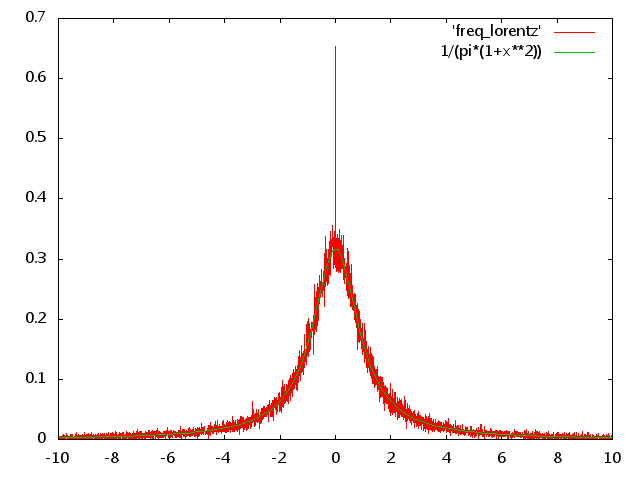
\includegraphics[width=4in]{lorentz.png}
\end{center}
可以看出和理论曲线非常一致 (中央的绿线是理论曲线).

然后用 \verb|gauss| 作为 \verb|pdist| 调用 \verb|count_freq|. 结果为:
\begin{center}
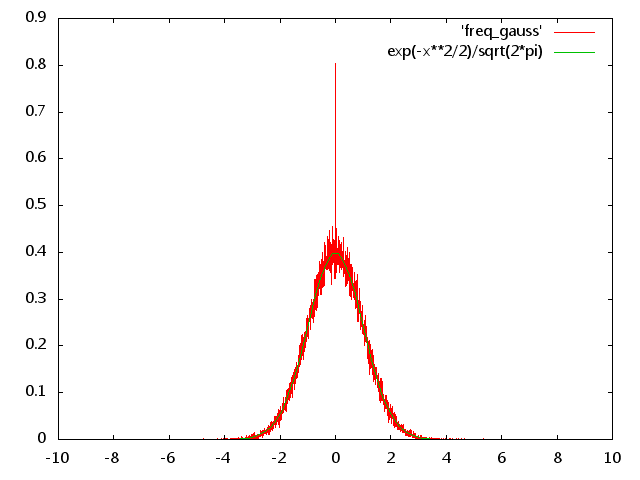
\includegraphics[width=4in]{gauss.png}
\end{center}
可以看出和理论曲线是非常一致的.

抽样效率: 理论上可以证明抽样效率为 $1/L \approx 0.657745$. 前面程序中计算出的值
为 $\input efficiency_gauss\relax$. 还是比较接近的.

\end{document}
